% *created  "Fri Jun  5 12:11:18 2020" *by "Paul E. Black"
% *modified "Wed Feb 16 09:36:57 2022" *by "Paul E. Black"

\documentclass[12pt]{article}
\usepackage{amsmath}
\usepackage{amsfonts}   % if you want the fonts
\usepackage{amssymb}    % if you want extra symbols
\usepackage{graphicx}   % need for figures
\usepackage{xcolor}
\usepackage{bm}
\usepackage{secdot}		
\usepackage{mathptmx}
\usepackage{float}
\usepackage[utf8]{inputenc}
\usepackage{textcomp}
\usepackage[hang,flushmargin,bottom]{footmisc} % footnote format

\usepackage{titlesec}
\titleformat{\section}{\normalsize\bfseries}{\thesection.}{1em}{}	% required for heading numbering style
\titleformat*{\subsection}{\normalsize\bfseries}

\usepackage{tocloft}	% change typeset, titles, and format list of appendices/figures/tables
\renewcommand{\cftdot}{}	
\renewcommand{\contentsname}{Table of Contents}
\renewcommand{\cftpartleader}{\cftdotfill{\cftdotsep}} % for parts
\renewcommand{\cftsecleader}{\cftdotfill{\cftdotsep}}
\renewcommand\cftbeforesecskip{\setlength{4pt}{}}
\addtolength{\cftfignumwidth}{1em}
\renewcommand{\cftfigpresnum}{\figurename\ }
\addtolength{\cfttabnumwidth}{1em}
\renewcommand{\cfttabpresnum}{\tablename\ }
\setlength{\cfttabindent}{0in}    %% adjust as you like
\setlength{\cftfigindent}{0in} 

\usepackage{enumitem}         % to control spacing between bullets/numbered lists

\usepackage[numbers,sort&compress]{natbib} % format bibliography 
\renewcommand{\bibsection}{}
\setlength{\bibsep}{0.0pt}

\usepackage[hidelinks]{hyperref}
\hypersetup{
	colorlinks = true,
urlcolor ={blue},
citecolor = {.},
linkcolor = {.},
anchorcolor = {.},
filecolor = {.},
menucolor = {.},
runcolor = {.}
pdftitle={},
pdfsubject={},
pdfauthor={},
pdfkeywords={}
}
\urlstyle{same}

\usepackage{epstopdf} % converting EPS figure files to PDF

\usepackage{fancyhdr, lastpage}	% formatting document, calculating number of pages, formatting headers
\setlength{\topmargin}{-0.5in}
\setlength{\headheight}{39pt}
\setlength{\oddsidemargin}{0.25in}
\setlength{\evensidemargin}{0.25in}
\setlength{\textwidth}{6.0in}
\setlength{\textheight}{8.5in}

\usepackage{caption} % required for Figure labels
\captionsetup{font=small,labelfont=bf,figurename=Fig.,labelsep=period,justification=raggedright} 

% put a light gray ``DRAFT'' diagonally across each page
\usepackage{draftwatermark}
\usepackage{datetime} % for \shortmonthname
\SetWatermarkText{DRAFT \number\day\ \shortmonthname}
% bigger percentage is closer to white
\SetWatermarkColor[gray]{0.9}
\SetWatermarkFontSize{3cm}
\SetWatermarkAngle{55}
\SetWatermarkHorCenter{11cm}

\usepackage{xcolor} % for colored text and backgrounds

%%%%%%%%%%% !!!!!! REQUIRED - FILL OUT METADATA FOR NISTIR HERE !!!!!!!! %%%%%%%%%%%%%%
%  	Report Number - fill in Report Number sent to you (see info below)
%   DOI Statement - fill in DOI sent to you 
%   Month Year - fill in Month and Year of Publication
%%%%%%%%%%%%%%%%%%%%%%%%%%%%%%%%%%%%%%%%%%%%%%%%%%%%%%%%%%%%%%%%%%%%%%%%%%%%%%%%%%%%%%
\newcommand{\pubnumber}{XXXX}
\newcommand{\DOI}{https://doi.org/10.6028/NIST.IR.XXXX}
\newcommand{\monthyear}{October 2020}
\newcommand{\paperTitle}{Vulnerability Test Suite Generator (VTSG) Version 3}

%%%%%%%%%%%%%%%%%%%%%%%%%%%%%%%%%%%%%%%%%%%%%%%%%%%%%%%%%%%%%%%%%%%%
%   	BEGIN DOCUMENT 
%%%%%%%%%%%%%%%%%%%%%%%%%%%%%%%%%%%%%%%%%%%%%%%%%%%%%%%%%%%%%%%%%%%%

% correct bad hyphenation here
\hyphenation{e-qua-tion}

% list of commands for horizontal spacing---and there are a LOT of them---and
% examples of each one
% https://tex.stackexchange.com/questions/74353/what-commands-are-there-for-horizontal-spacing

% to wrap paragraph in table cells
\usepackage{makecell}

% typeset C#
% According to the ECMA-334 C# Language Specification, 5th
% Edition, Sec. 5, Acronyms and abbreviations, ``The name 
% C# is written as the LATIN CAPITAL LETTER C (U+0043) followed 
% by the NUMBER SIGN # (U+0023).'' \cite{ECMA-CSharp2017}
% https://www.ecma-international.org/publications/standards/Ecma-334.htm
% Dec 2017, Accessed: 12 June 2020
\newcommand{\CSharp}{C{\fontseries{b}\selectfont\#}}
% another possibility is C\nolinebreak\#\



\begin{document}
	\urlstyle{rm} % Format style of \url   

%%%%%%%%%%%%%%%%%%%%%%%%%%%%%%%%%%%%%%%%%%%%%%%%%%%%%%%%%%%%%%%%%%%%
%   Cover Page is REQUIRED and must contain the information 
%	displayed here, at a minimum. Additional artwork may be included 
%	(e.g., official project/conference logo, etc.).
%	Pub Number automated based on metadata
%%%%%%%%%%%%%%%%%%%%%%%%%%%%%%%%%%%%%%%%%%%%%%%%%%%%%%%%%%%%%%%%%%%%
\begin{titlepage}
\begin{flushright}
%%%%%%%%%%%%%%%%%%%%%%%%%%%%%%%%%%%%%%%%%%%%%%%%%%%%%%%%%%%%%%%%%%%%
% 	Automated based on metadata - delete if not applicable
%%%%%%%%%%%%%%%%%%%%%%%%%%%%%%%%%%%%%%%%%%%%%%%%%%%%%%%%%%%%%%%%%%%%
\LARGE{\textbf{NISTIR \pubnumber}}\\
\vfill
%%%%%%%%%%%%%%%%%%%%%%%%%%%%%%%%%%%%%%%%%%%%%%%%%%%%%%%%%%%%%%%%%%%%
%	Title 
%%%%%%%%%%%%%%%%%%%%%%%%%%%%%%%%%%%%%%%%%%%%%%%%%%%%%%%%%%%%%%%%%%%%
\Huge{\textbf{\paperTitle}}\\
    \vfill
%%%%%%%%%%%%%%%%%%%%%%%%%%%%%%%%%%%%%%%%%%%%%%%%%%%%%%%%%%%%%%%%%%%%
%	Authors - add complete list of authors, affiliations will be 
%   added on title page
%%%%%%%%%%%%%%%%%%%%%%%%%%%%%%%%%%%%%%%%%%%%%%%%%%%%%%%%%%%%%%%%%%%%
    \large Paul E. Black \\
    \large William Mentzer\\
    \large Elizabeth Fong \\
    \large Bertrand Stivalet
\vfill
%%%%%%%%%%%%%%%%%%%%%%%%%%%%%%%%%%%%%%%%%%%%%%%%%%%%%%%%%%%%%%%%%%%%
%	The DOI is automated based on metadata.	
%%%%%%%%%%%%%%%%%%%%%%%%%%%%%%%%%%%%%%%%%%%%%%%%%%%%%%%%%%%%%%%%%%%%
\normalsize This publication is available free of charge from:\\
\DOI\\
\vfill
%%%%%%%%%%%%%%%%%%%%%%%%%%%%%%%%%%%%%%%%%%%%%%%%%%%%%%%%%%%%%%%%%%%%
%	NIST LOGO - keep as-is
%%%%%%%%%%%%%%%%%%%%%%%%%%%%%%%%%%%%%%%%%%%%%%%%%%%%%%%%%%%%%%%%%%%%


\includegraphics[width=0.3\linewidth]{NIST-logo.eps}\\ 
 
  
\end{flushright}
\end{titlepage}
\begin{titlepage}
%%%%%%%%%%%%%%%%%%%%%%%%%%%%%%%%%%%%%%%%%%%%%%%%%%%%%%%%%%%%%%%%%%%%
%	Title Page is REQUIRED
%%%%%%%%%%%%%%%%%%%%%%%%%%%%%%%%%%%%%%%%%%%%%%%%%%%%%%%%%%%%%%%%%%%%
\begin{flushright}
%%%%%%%%%%%%%%%%%%%%%%%%%%%%%%%%%%%%%%%%%%%%%%%%%%%%%%%%%%%%%%%%%%%%
%   Publication Series & Number - automated
%%%%%%%%%%%%%%%%%%%%%%%%%%%%%%%%%%%%%%%%%%%%%%%%%%%%%%%%%%%%%%%%%%%%
\LARGE{\textbf{NISTIR \pubnumber}}\\
\vfill 
%%%%%%%%%%%%%%%%%%%%%%%%%%%%%%%%%%%%%%%%%%%%%%%%%%%%%%%%%%%%%%%%%%%%
%	Title 
%%%%%%%%%%%%%%%%%%%%%%%%%%%%%%%%%%%%%%%%%%%%%%%%%%%%%%%%%%%%%%%%%%%%
\Huge{\textbf{\paperTitle}}\\
    \vfill
%%%%%%%%%%%%%%%%%%%%%%%%%%%%%%%%%%%%%%%%%%%%%%%%%%%%%%%%%%%%%%%%%%%%
%	Author Order and Grouping. Always identify the primary author/creator first
% (s/he does not have to be a NIST author). For publications with multiple authors,
% group authors by their organizational affiliation. The organizational groupings and
% the names within each grouping should generally be ordered by decreasing level of
% contribution.
%	For non-NIST authors, list their city and state below their organization name.
%	For NIST authors, include the Division and Laboratory names (but do not
% include their city and state).
%%%%%%%%%%%%%%%%%%%%%%%%%%%%%%%%%%%%%%%%%%%%%%%%%%%%%%%%%%%%%%%%%%%%
    \normalsize 
    Paul E. Black\\
     \textit{Software and Systems Division}\\
     \textit{Information Technology Laboratory}\\
     \vspace{12pt}
    William Mentzer\\
     \textit{California State University}\\
     \textit{San Bernardino, California}\\
     \vspace{12pt}
    Elizabeth Fong \\
     \textit{affiliation}\\
     \textit{location}\\
     \vspace{12pt}
    Bertrand Stivalet \\
     \textit{affiliation}\\
     \textit{location}
\vfill
%%%%%%%%%%%%%%%%%%%%%%%%%%%%%%%%%%%%%%%%%%%%%%%%%%%%%%%%%%%%%%%%%%%%
%   DOI Statement - automated
%%%%%%%%%%%%%%%%%%%%%%%%%%%%%%%%%%%%%%%%%%%%%%%%%%%%%%%%%%%%%%%%%%%%
\normalsize This publication is available free of charge from:\\
\DOI\\
\vfill
%%%%%%%%%%%%%%%%%%%%%%%%%%%%%%%%%%%%%%%%%%%%%%%%%%%%%%%%%%%%%%%%%%%%
%   Date - Month and Year - automated
%%%%%%%%%%%%%%%%%%%%%%%%%%%%%%%%%%%%%%%%%%%%%%%%%%%%%%%%%%%%%%%%%%%%
\normalsize \monthyear
\vfill
%%%%%%%%%%%%%%%%%%%%%%%%%%%%%%%%%%%%%%%%%%%%%%%%%%%%%%%%%%%%%%%%%%%%
%  Department of Commerce LOGO - leave as-is
%%%%%%%%%%%%%%%%%%%%%%%%%%%%%%%%%%%%%%%%%%%%%%%%%%%%%%%%%%%%%%%%%%%%	


\includegraphics[width=0.18\linewidth]{DoC-logo.eps}\\ 
 \vfill
%%%%%%%%%%%%%%%%%%%%%%%%%%%%%%%%%%%%%%%%%%%%%%%%%%%%%%%%%%%%%%%%%%%%
%  Department of Commerce & NIST Leadership 
%	will be updated as changes occur
%%%%%%%%%%%%%%%%%%%%%%%%%%%%%%%%%%%%%%%%%%%%%%%%%%%%%%%%%%%%%%%%%%%%
\footnotesize U.S. Department of Commerce\\ 
\textit{Wilbur L. Ross, Jr., Secretary}\\
\vspace{10pt}
National Institute of Standards and Technology\\ 
\textit{Walter Copan, NIST Director and Undersecretary of Commerce for Standards and Technology}  
\end{flushright}
\end{titlepage}
\begin{titlepage}
%%%%%%%%%%%%%%%%%%%%%%%%%%%%%%%%%%%%%%%%%%%%%%%%%%%%%%%%%%%%%%%%%%%%
%   Disclaimer/CODEN page - required
%%%%%%%%%%%%%%%%%%%%%%%%%%%%%%%%%%%%%%%%%%%%%%%%%%%%%%%%%%%%%%%%%%%%
\begin{flushright}
\footnotesize  Certain commercial entities, equipment, or materials may be identified
in this document in order to describe an experimental procedure or concept
adequately. Such identification is not intended to imply recommendation or
endorsement by the National Institute of Standards and Technology, nor is it intended
to imply that the entities, materials, or equipment are necessarily the best
available for the purpose.\\

\vfill
%%%%%%%%%%%%%%%%%%%%%%%%%%%%%%%%%%%%%%%%%%%%%%%%%%%%%%%%%%%%%%%%%%%%
%   This section automated - do not change
%%%%%%%%%%%%%%%%%%%%%%%%%%%%%%%%%%%%%%%%%%%%%%%%%%%%%%%%%%%%%%%%%%%%
\normalsize \textbf{National Institute of Standards and Technology \\ Internal Report \pubnumber\\ 
Natl. Inst. Stand. Technol. Intern. Rep. \pubnumber, \pageref{LastPage} pages (\monthyear)} \\
\vspace{12pt}
\textbf{This publication is available free of charge from: \DOI}
\vfill
\end{flushright}
\end{titlepage}
%%%%%%%%%%%%%%%%%%%%%%%%%%%%%%%%%%%%%%%%%%%%%%%%%%%%%%%%%%%%%%%%%%%%
%   Start front matter - page number starts with "i"
%%%%%%%%%%%%%%%%%%%%%%%%%%%%%%%%%%%%%%%%%%%%%%%%%%%%%%%%%%%%%%%%%%%%
\pagenumbering{roman}

\section*{Abstract}
\normalsize
The Vulnerability Test Suite Generator (VTSG) can create vast numbers of
synthetic programs with and without specific flaws or vulnerabilities.
It was designed by the Software Assurance Metrics and Tool Evaluation (SAMATE) team
and originally implemented by students from TELECOM Nancy.
The latest version is structured to be able to generate vulnerable and nonvulnerable
synthetic programs expressing specific flaws in \emph{any} programming language.
It has libraries to generate PHP, \CSharp, and Python programs.
This document may help if you are trying to generate test cases written in 
PHP, \CSharp, or Python or if you are modifying VTSG Version 3 to generate test 
cases in other programming languages.

\section*{Key words}
\normalsize Software assurance; static analyzer; test case generator; 
software vulnerabilities.

% push next part to the bottom of the page
\vfill

This document was written at the National Institute of Standards and
Technology by employees of the Federal Government in the course of
their official duties.  Pursuant to title 17 Section 105 of the United
States Code this is not subject to copyright protection and
is in the public domain.


We would appreciate acknowledgment if this document is used.

\pagebreak
%%%%%%%%%%%%%%%%%%%%%%%%%%%%%%%%%%%%%%%%%%%%%%%%%%%%%%%%%%%%%%%%%%%%
%   Table of Contents is required
% 	List of Tables & Figures required if more than 5 tables/figures
%%%%%%%%%%%%%%%%%%%%%%%%%%%%%%%%%%%%%%%%%%%%%%%%%%%%%%%%%%%%%%%%%%%%
\begin{center}
\tableofcontents
%\listoftables
%\listoffigures
\end{center}
\pagebreak
%%%%%%%%%%%%%%%%%%%%%%%%%%%%%%%%%%%%%%%%%%%%%%%%%%%%%%%%%%%%%%%%%%%%
%   Start body of text - page number starts with "1"
%%%%%%%%%%%%%%%%%%%%%%%%%%%%%%%%%%%%%%%%%%%%%%%%%%%%%%%%%%%%%%%%%%%%

\newpage

\section{Introduction}
\pagenumbering{arabic}

{\Large We will use vulnerability, instead of flaw or weakness. other SAMATE documents use ``weakness''.}

The Vulnerability Test Suite Generator (VTSG) generates collections 
of vulnerable and non-vulnerable
synthetic programs expressing specific flaws.  
The programs can be used as 
test cases to evaluate static analyzers. 
Each test case targets one flaw. There are two types of test cases:
cases with flawed code, leading to a vulnerability, and cases that
have similar behavior, but have the flaw corrected. That is, no
vulnerability.  Exactly corresponding vulnerable and non-vulnerable
cases could, in theory, be generated. However, since each test case
is generated separately, there is no exact correspondence between 
cases.

The generator is written in Python 3.

\subsection{History} 

VTS version 1 only generated \CSharp\ programs. VTS version 2 generated PHP
programs~\cite{StivaletFongVTSPHP2016} in addition.  Version 2 is more
customizable to generate other programming languages.
VTSG version 3 (V3) systematically maintains indentation, so also
generates Python programs.  VTSG V3 produces manifest files in the
Static Analysis Results Interchange Format (SARIF) 
Version 2.1.0~\cite{SARIF2.1.0} format.

Readers can download the PHP and \CSharp\ test cases generated 
by earlier versions from NIST’s Software Assurance Reference 
Dataset (SARD):
\href{http://samate.nist.gov/SARD}{http://samate.nist.gov/SARD}

The global project can be found at: \href{https://github.com/usnistgov/VTSG}{https://github.com/usnistgov/VTSG}\\


\subsection{Install Supporting Packages}

\noindent The following instructions are provided for users, who may not have these packages already installed on their Linux machines. Users who already have these packages may skip this section.

\noindent To download files from Github, one must install the \emph{Git} package. Use the following command to install git:

\begin{verbatim}
    sudo apt-get install git    
\end{verbatim}

\noindent To execute Python source code, one must install the \emph{pip Python} package manager. Use the following command to install it:

\begin{verbatim}
    sudo apt-get install python-pip
\end{verbatim}

\noindent VTSG is written in Python 3, so Python 3 must be installed, too.
Use the following command to install Python 3:

\begin{verbatim}
    sudo apt-get install python3
\end{verbatim}

\noindent In addition, the \emph{pip Python 3} package manager must be installed, using the following command:

\begin{verbatim}
    sudo apt-get install python3-pip
\end{verbatim}

\noindent To validate \CSharp\ test cases, \emph{mono} and \emph{mcs} must be installed. The Mono project created \emph{mono} as an open source platform, which implements the .NET Framework. Class libraries and \CSharp\ compilation are enabled by \emph{mcs} (\href{http://github.com/mono/mono}{http://github.com/mono/mono}).

\noindent Use the following command to obtain mono-complete:

\begin{verbatim}
    sudo apt-get install mono-complete
\end{verbatim}

\noindent Type the following command to obtain \emph{mcs}:

\begin{verbatim}
    sudo apt-get install mcs
\end{verbatim}

\subsection{Install VTSG}

\noindent To copy the generic VTSG from GitHub to a local Linux machine, change to a
directory under which you want VTSG installed.

\noindent Returning to the GitHub website, one will see a green box, labelled ``Clone or download''. Click on it and use the clipboard tab to copy the web URL.

\noindent Type the following command to copy the source code and other material to the local directory:

\begin{verbatim}
    git clone https://github.com/usnistgov/VTSG.git
\end{verbatim}

\noindent If one types the \verb|ls -a| command, one will see that the \textbf{VTSG} directory was created.

\noindent Go to that directory, using the following command:

\begin{verbatim}
    cd VTSG
\end{verbatim}

\noindent To install the dependencies, use the following command:

\begin{verbatim}
    pip3 install --user -r requirements.txt
\end{verbatim}


\subsection{Users}

There are two groups who will typically use VTSG. The first group comprises people
requiring test cases written in PHP, \CSharp, or Python to evaluate a static
analyzer. These users must know how to invoke VTSG with command line interface and
retrieve the appropriate sample from the generated and categorized folders.

The second targeted audience of the VTSG is comprised of people wishing to generate
test cases using a programming language other than the languages currently
supported. The second group of users must use the template to construct the program
using the XML tags, execute VTSG with command line interface or another input method,
and retrieve the samples from the generated and categorized file folders.

\subsection{Vulnerabilities Supported by VTSG}

Vulnerabilities are encoded in the language files, see Sec.~\ref{sec:source files}.
Some of the OWASP Top 10~\cite{OWASPTop10-2017} and
Common Weakness Enumerations (CWEs)~\cite{CWE} are encoded.  The following list shows
the vulnerabilities currently in each language:
\begin{itemize}
    \item SQL Injection (\CSharp, PHP)
    \item XPath Injection (\CSharp)
    \item LDAP Injection (\CSharp)
    \item OS Command Injection (\CSharp)
    \item Path traversal (\CSharp)
\end{itemize}

\section{Command Line Interface}
\label{sec:command line interface}

For users who wish to generate PHP or \CSharp\ test suites, a command line interface
can generate all test cases or a specific group of test cases based on several
options.  For example, the user can generate vulnerable or non-vulnerable test cases
based on selected OWASP categories or CWE weaknesses.  The user must specify the
programming language.  The invocation command looks like this:
\begin{verbatim}
$ python3 vtsg.py -l {php,cs,py} <options>
\end{verbatim}

% Overleaf complains that textcomp doesn't provide \textlangle
% and \textrangle in the font family.  So we define our own.
\newcommand{\texlangle}{$\langle$}
\newcommand{\texrangle}{$\rangle$}
Where \texlangle options\texrangle\ can be selected from 
Table~\ref{tab:command line options}.

\begin{table}[H]
\centering
\begin{tabular}{|l|l|}
\hline
-h --help & Show help and quit \\
\hline
--version & Show version number and quit \\
\hline
-l LANGUAGE 
--language=LANGUAGE &
\makecell[l]{Language of generated cases. \\
Currently one of php, for PHP \\
cases, cs, for \CSharp\ cases, or py, \\
for Python cases. 
See Sec.~\ref{sec: directory structure}.} \\
\hline
\makecell[l]{-f FLAW\_GROUP[,FLAW\_GROUP]* \\
--flaw-group=FLAW\_GROUP[,FLAW\_GROUP]*} &
\makecell[l]{Only generate cases with \\
vulnerabilities from the specified \\
group(s). See Sec.~\ref{sec:sink modules}} \\
\hline
-c CWE[,CWE]*
--cwe=CWE[,CWE]* &
\makecell[l]{Only generate cases with vulner- \\
abilities from the specified CWE(s). \\
See Sec.~\ref{sec:sink modules}} \\
\hline
-s
--safe & 
Only generate non-vulnerable cases \\
\hline
-u
--unsafe & 
Only generate vulnerable cases \\
\hline
-r DEPTH
--depth=DEPTH &
\makecell[l]{Maximum nested depth of \\
complexities (Default: 1) See \\ 
Sec.~\ref{sec:depth of complexities}} \\
\hline
-g NUMBER
--number-generated=NUMBER &
\makecell[l]{Maximum number of sink, filter, \\
input (and exec query) combina- \\
tions to generate. (Default: -1, \\
meaning all) See below for \\
explanation.} \\
\hline
-d
--debug &
\makecell[l]{{\Large Not Used --} \\
{\Large Remove from code}} \\
\hline
\end{tabular}
\caption{Options for Command Line Invocation}
\label{tab:command line options}
\end{table} 

\subsection{Explanation of Options}

The default is to generate both the unsafe (buggy or vulnerable)
test cases and the safe (not buggy) test cases.  You can select
either only safe (-s) or only unsafe (-u) cases.  The options are
mutually exclusive.

The -g (number-generated) option has limited utility.  When the
specified number of sink, filter, input (and exec query, if needed)
combinations are generated, VTSG terminates.  The default, -1,
means generate all combinations.

Each combination of sink, filter, input, and exec query is elaborated
with DEPTH nested complexities.  Suppose there are 5 complexities
and VTSG is invoked with \verb|-r 2|.  Each combination will have
1 (no complexities) + 5 (each complexity, not nested) + 
25 (each complexities nested within every complexity) = 31 test cases.  
Hence VTSG may generate \emph{far} more test cases than the number
given with the -g option.

\subsection{Example Invocations}

Show the help message:
\begin{verbatim}
$ python3 vtsg.py --help
\end{verbatim}

Generate all PHP test cases:
\begin{verbatim}
$ python3 vtsg.py -l php
\end{verbatim}

Generate a \CSharp\ (\verb|-l cs|) test suite made of non-vulerable (unsafe) test
cases (\verb|-u|) with SQL injection vulnerabilities (\verb|--cwe=89|) 
with up to 3 nested levels of complexity (\verb|-r 3|).
\begin{verbatim}
$ python3 vtsg.py -l cs -r 3 --cwe=89 -u
\end{verbatim}
 
\section{Overview of VTSG}

\begin{figure}[htbp]
  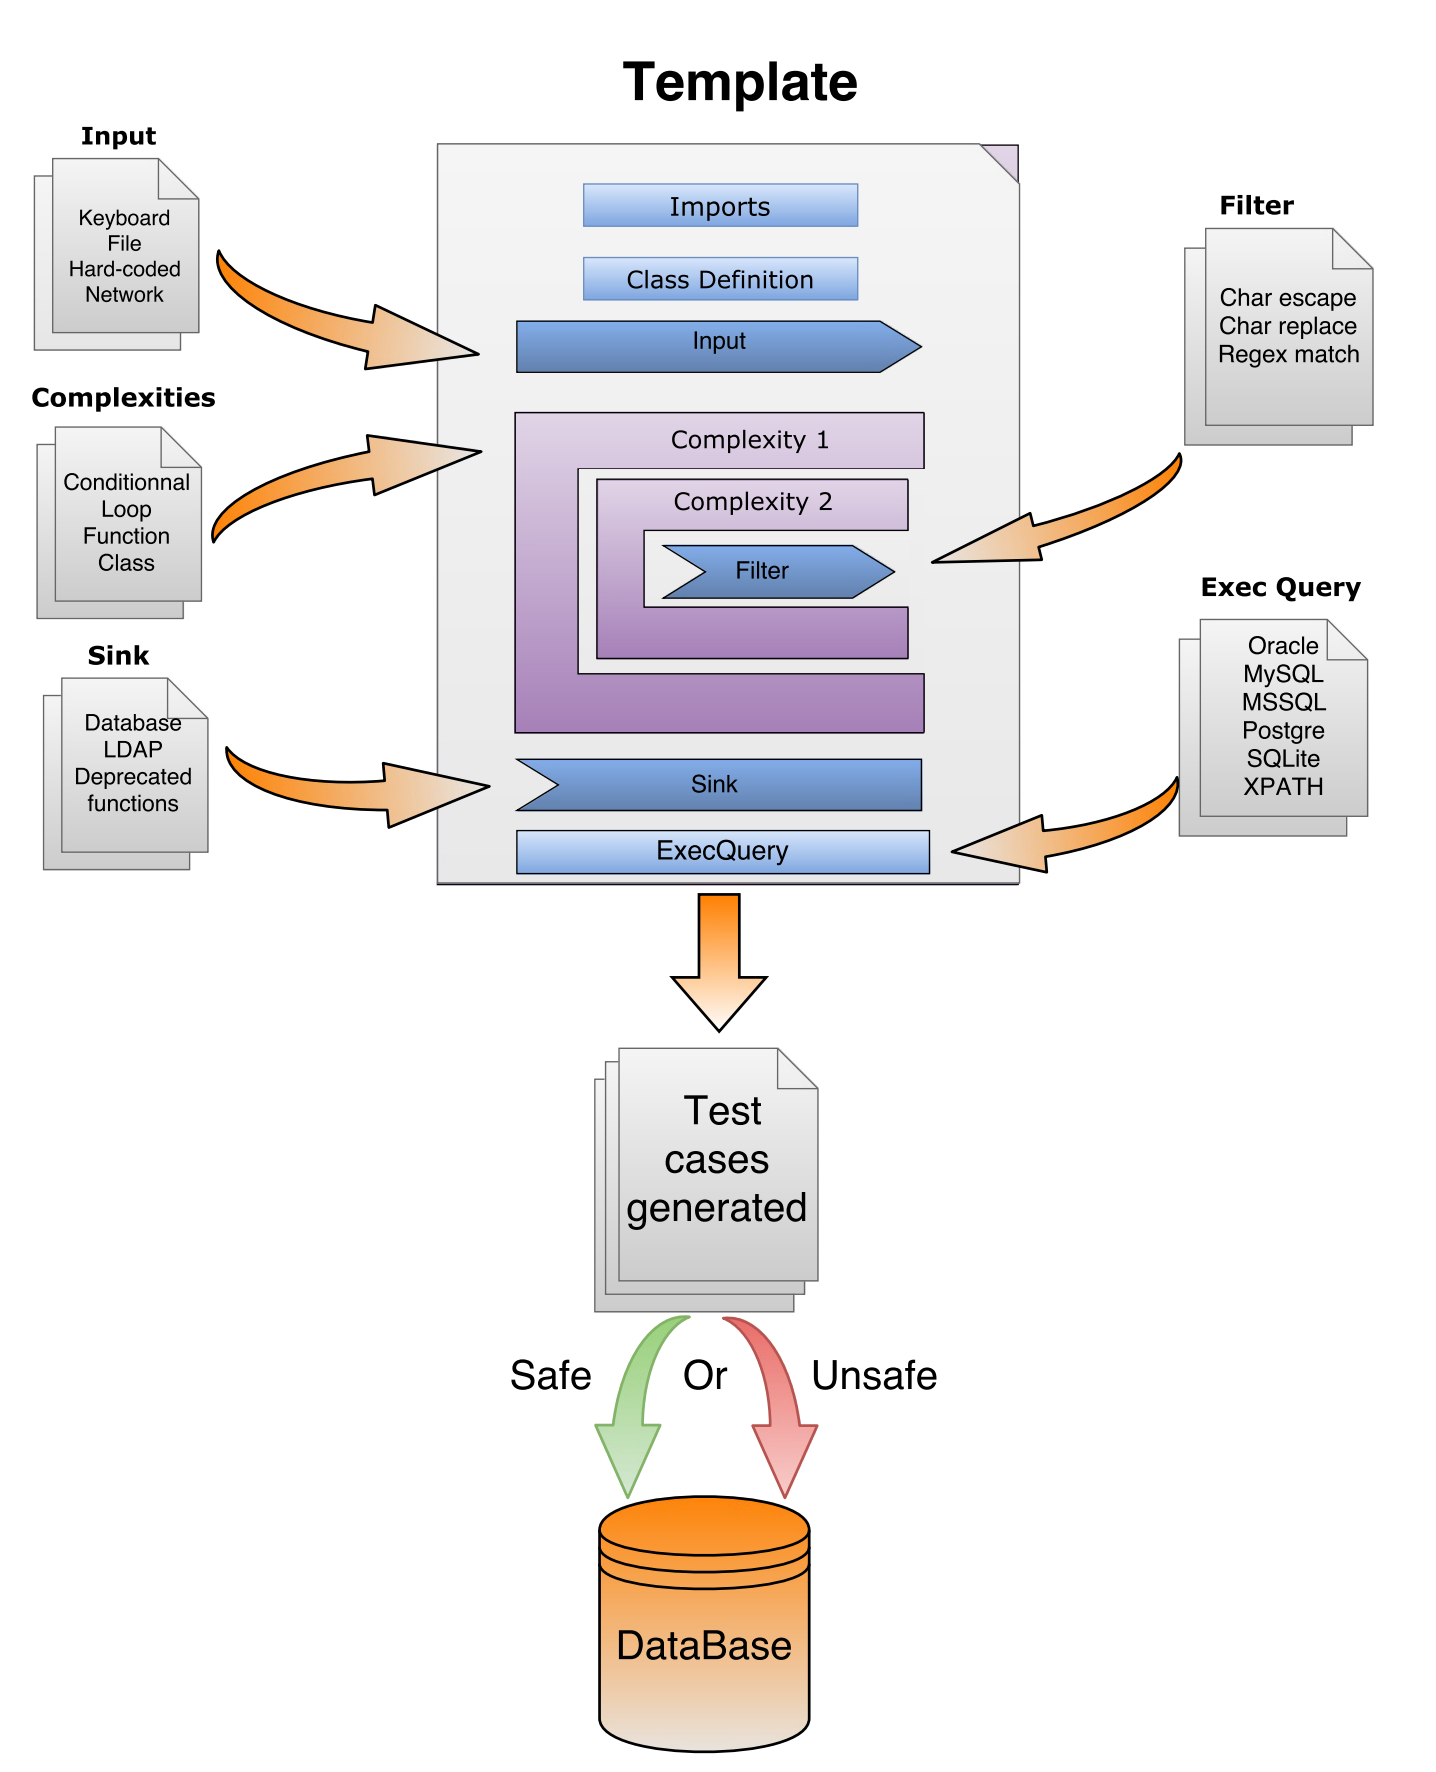
\includegraphics[width=1\linewidth]{fig_VTSG_overview.png}
  \caption{Overview of VTSG test case generation process. The Template
  specifies how pieces are assembled. The Input, Filter, Complexities,
  Sink, and ExecQuery modules provide alternative code.  
  An example of
  a generated test case is in 
  Figs.~\ref{fig:example main file} and 
  \ref{fig:example aux file}.}
  \label{fig:VTS operation overview}
\end{figure}

{\large Explain that there are TWO structures. The structure of test
  cases generated and the structure of VTSG.  Make it clear when each
  is being explained.}

\subsection{Overview of Test Case Generation}

VTSG V3 generates test cases from information in Template, Input,
Filter, Sink, Complexity and ExecQuery files 
(see Fig.~\ref{fig:VTS operation overview}):
\begin{itemize}
 \item Template is the overall structure of each program.
 \item Input is the source of untrusted data in the program, e.g., 
 command line, variable, files, and form methods.
 \item Filtering filters the input with sanitization functions, 
 casting, deprecated functions, or simply no filtering.
 \item Sink is where a sensitive operation, such as a database query, 
 is executed with potentially untrusted input and where the 
 vulnerability is triggered.
 \item ExecQuery is an additional piece of code that is mandatory to 
 trigger the vulnerability.
 \item Complexity is how the data flow and control flow are 
 implemented in the structure of the program.
\end{itemize}
The content of these files is detailed in
Sec.~\ref{sec:source files}.
Details of the generation process are explained in
Sec.~\ref{sec: generation detail}.

\subsection{VTSG Directory Structure}
\label{sec: directory structure}

All these types of files are kept in a \verb|templates| subdirectory.
Under this is one subdirectory for each language.  VTSG chooses the
directory based on the language selected in the \verb|-l| command line
option.  Each language subdirectory has six files for that language.
The files are \verb|file_template.xml|, \verb|input.xml|, 
\verb|complexities.xml|, \verb|filtering.xml|, \verb|sink.xml|,
and \verb|exec_queries.xml|.  To add another language,
simply create a subdirectory for that language with the six description
files.

The \verb|templates| directory has \verb|file_rights.txt|, which is
copied into each generated test case to declare license rights and
authorship, see Sec.~\ref{sec: file template}, and a 
\verb|dtd| subdirectory, which has a document type definition (DTD) 
for Template, Input, Filter, and all other XML files.


\subsection{Generation Process}
\label{sec: generation detail}

Each test case is constructed based on the file Template, as shown
in Fig.~\ref{fig:VTS operation overview}. Test cases are 
programs in a specific program language.  
Each test case is generated by
assembling the modules according to the Template.  The
template may direct construction of a simple test case with just
an Input, a Filter, and a Sink.  
The Filtering code may be embedded in data and control flow
Complexity code.

VTSG generates test cases with two broad steps.  First, VTSG selects
Input, Filter, Complexities, Sink, and ExecQuery modules that are
compatible with each other and consistent with any flaw group or
CWE constraints the user gives on the command line.  Second, VTSG
composes test case source code from the selected modules, 
synthesizing variable and functions names, and writes the file(s).

The code structure is roughly
\begin{verbatim}
    for each specified sink
        for each filter
            for each input
                for each exec query
                    for up to DEPTH combinations of each complexity
                        compose a test case with these modules
\end{verbatim}
The code is more complicated because only compatible modules are 
selected.
In addition, some sinks do not need any input or filtering at all,
see Sec.~\ref{sec:sink modules}.
The
code is structured as a series of function calls to allow types
of modules to be skipped.  Here is a slightly more detailed
overview of those steps:
\begin{verbatim}
    for each sink:
        if sink is specified:
            if input is needed:
                select_filtering()
            else:
                select_exec_query()
    
    def select_filtering():
        for each filter:
            if filter is compatible with sink:
                select_input()
    
    def select_input()
        for each input:
            if input is compatible with filter:
                select_exec_query()

    def select_query()
        if sink needs exec_query:
            for each exec_query:
                if exec_query is compatible with sink:
                    select_complexity_or_compose()
        else:
            select_complexity_or_compose()

    def select_complexity_or_compose():
        if input_type is not none:
            recursive_select_complexity()
        else:
            compose()

    ... and so forth
\end{verbatim}

The \emph{test\_suite\_gen.py} script creates a new object of the
\emph{Generator} class. 
The program iterates through all sink modules, selecting those
specified by the user, see
Sec.~\ref{sec:command line interface}, 
or all of them if the user does not specify. It subsequently
selects filters then inputs then exec queries and complexities
that are compatible with the currently selected sink module.

When VTSG has selected a set of modules, it begins composing
the code in them to generate the source code for a test case.
The process of composing modules to generate source code is
based on XML metadata tags.
After the imports and class definition declaration for the 
specific program
language, the ``Input'' metadata \texlangle code\texrangle\  portion 
is added to the test case.  
The \texlangle input\_type\texrangle\ and 
\texlangle output\_type\texrangle\ 
must be consistent with the ``Filtering'' and ``Sink'' XML tags.  The 
``Filtering'' metadata \texlangle code\texrangle\ portion, plus its 
\texlangle flaw type\texrangle\ and safety indicator, are added to 
the test case.  Next, the ``Sink'' metadata 
\texlangle code\texrangle\ portion 
is added to the test case.  Finally, the ``ExecQuery'' type is 
noted and the 
\texlangle code\texrangle\ portion of the ``ExecQuery'' is added 
to the 
test case.  The test case is written to a file.  
The location of the file is
described in Sec.~\ref{sec: test suite directory structure}.
Section~\ref{sec:case file name} describes how VTSG names the file.

VTSG generates many different test cases, both with and without
flaws, with various control flow complexities.  After VTSG finishes
generating each vulnerability category, it displays how many safe (non-vulnerable)
and unsafe (vulnerable) test cases it produced.
VTSG generates hundreds of test cases in minutes.

VTSG is built to generate test cases with all consistent combinations
of modules for the flaw groups and CWEs specified in the invocation.
If VTSG is invoked with flaw groups (\verb|-f|) or CWEs (\verb|-c|),
only sinks satisfying those specified are used.
If no flaw groups are specified, all flaw groups are used.  
If no CWEs are specified, all CWEs are used.

\label{sec:depth of complexities}
The depth command line option, \verb|-r| or \verb|--depth|, 
specifies the
most nested flow control complexities produced.
VTSG generates test cases with all complexities up to the depth
indicated.
For example, the default depth, 1, leads VTSG to generate all
test cases with no flow complexities and all test cases with 
one complexity.  The option \verb|-r 2| leads VTSG to generate
all cases with no complexities, all cases with one complexity, 
and all cases with two nested complexities.
See Sec.~\ref{sec:code complexities} for an example of three 
nested control flow complexities.

\subsection{Code Complexities}
\label{sec:code complexities}

In theory, a static analysis tool only needs to process a few lines of
code that
embody the vulnerability. In practice, a tool must analyze most 
of the program,
noting its control and data flows, to accurately track data and
determine the
conditions when the code with weaknesses may be executed.
Code complexities are constructs that may confuse static 
analysis tools.  
Each code complexity element can have many different attributes
associated with it.
They are combined and nested to create real source code.  
For example, the value 
of an expression may come from a constant, a single variable, 
some arithmetic 
combination, or the return value of a function call.  
Flow of control may be
influenced by loops, conditionals, and functions calls.  
Also, there could be many 
layers or depths of such nesting structures.  

The Complexity identifications currently available for PHP 
and \CSharp\ are listed in 
Table~\ref{tab:complexity IDs} in the Appendix.

Here is an example code complexity from \verb|cwe_89__I_shell_commands__F_no_|\\ 
\verb|filtering__S_select_from-concatenation_simple_quote__EQ_mysql__3-2.5-| \\ 
\verb|9-21_File1.cs|: \\
{\texttt
{\colorbox{yellow}{if((Math.Pow(4, 2)<=42))\{}}\\
\hspace*{2em}{\colorbox{green}{switch(6)\{}}\\
\hspace*{4em}{\colorbox{green}{case(6):}}\\
\hspace*{6em}{\colorbox{cyan}{Class\_489618 var\_489618 = new Class\_489618(tainted\_5);}}\\
\hspace*{6em}{\colorbox{cyan}{tainted\_6 = var\_489618.get\_var\_489618();}}\\
\hspace*{6em}tainted\_7 = tainted\_6;\\
\hspace*{6em}{\colorbox{green}{break;}}\\
\hspace*{4em}{\colorbox{green}{default:}}\\
\hspace*{6em}{\colorbox{green}{break;}}\\              
\hspace*{2em}{\colorbox{green}{\}}}\\
{\colorbox{yellow}{\}else\{}}\\
\hspace*{2em}{\colorbox{yellow}{\{\}}}\\
{\colorbox{yellow}{\}}}
}


The above has complexity depth 3, note \verb|__3| near the end of 
the file
name. They correspond to:\\
{\colorbox{yellow}{Level 1 is the conditional}} id = 2.5\\
\hspace*{2em}{\colorbox{green}{Level 2 is the switch statement}} id = 9\\
\hspace*{4em}{\colorbox{cyan}{Level 3 is the call of a method from a Class defined in a different file}}, id = 21.

\section{Template, Input, Filter, Sink, Exec\_Query, and Complexity Files}
\label{sec:source files}

These XML files are required when adding new functionality to VTSG.
There 
are a few XML-specific caveats that must be paid attention to when 
creating these files. 
Table~\ref{tab:XML escapes} lists the symbols that may cause errors 
during the process and the XML equivalent replacement necessary to 
complete the
task without error.

\begin{table}[H]
\centering
\begin{tabular}{|c|l|}
\hline
\textbf{Character} & \textbf{Replacement} \\
\hline
 \verb|<| & \&lt; \\
\hline
 \verb|>| & \&gt; \\
\hline
 \verb|"| & \&quot; \\
\hline
 \verb|'| & \&apos; \\
\hline
 \verb|&| & \&amp; \\
\hline
\end{tabular}
\caption{Replacement sequences for characters that are treated 
in a special way in XML files.}
\label{tab:XML escapes}
\end{table}

Characteristics of modules and their information are stored in 
XML files.  
This section describes the structure of each type of module and 
the meaning
of each element and its tags.

Most of the file types have an example followed by
an explanation of what it does and what it generates at the end.

Each language directory has one file for each type. That is, 
one \verb|file_template.xml| file, one \verb|input.xml| file, 
one \verb|filtering.xml| file, one \verb|complexities.xml| file,
one \verb|sink.xml| file, and one \verb|exec_queries.xml| file.

The \verb|input.xml|, \verb|filtering.xml|, \verb|complexities.xml|,
\verb|exec_queries.xml|, and \verb|sink.xml| files may have many
modules in them.  For example, \verb|input.xml| typically has
many input modules, Sec.~\ref{sec: input module}, each getting 
input from a different source.

\subsection{File Template}
\label{sec: file template}

\begin{verbatim}
<template type="" name="">
    <file_extension></file_extension>
    <comment>
        <open></open>
        <close></close>
        <inline></inline>
    </comment>
    <syntax>
        <statement_terminator></statement_terminator>
    </syntax>
    <namespace></namespace>
    <variables prefix="" import_code="using {{import_file}};">
        <variable type="" code="" init=""/>
    </variables>
    <imports>
        <import></import>
    </imports>
    <code></code>
</template>
\end{verbatim}

\begin{itemize}
    \item name: Programming language name, e.g., PHP, CSharp, 
    or Python. This appears in the manifest.
    It is also the subdirectory under the TestSuite directory 
    where all the generated test cases are placed.

    \item file\_extension: Extension of the generated files.

    \item comment: Strings indicating comments.
    \begin{itemize}
        \item open: string to begin a comment, which may span many lines
        \item close: string to end a comment, which may span many lines
        \item inline: string to begin a one-line comment
    \end{itemize}
    
    \item syntax: Other language-specific syntax.
    \begin{itemize}
        \item statement\_terminator: string to show the end of 
        a statement.
        This is semicolon
        \verb|<statement_terminator>;</statement_terminator>|
        in PHP, C, Java, \\ and \CSharp. Python does not have 
        a terminator, so this is the empty string: \\
        \verb|<statement_terminator></statement_terminator>|.
    \end{itemize}
    
    \item namespace: Namespace name, if applicable

    \item variables: Information variable names and types and how
    to include libraries.
    \begin{itemize}
        \item prefix: Any prefix required for variable name, 
        \$ for PHP.
        Leave it blank if not required.

        \item import\_code: Code to include a library. The code
        should have the placeholder \verb|{{import_file}}|.
        For example, \verb|#include <{{import_name}}>|).
        
        \item variable: Defines each variable type and how it will 
        be used.
        \begin{itemize}
        \item type: Names the type. This string 
        does not appear in the test case code.  It tells VTSG
        the type of variable that is being used.  The input\_type
        and output\_type in Input, Filter, and Sink modules use
        this string.

        \item code: A piece of code declaring the type of the variable. For 
        some languages, such as PHP and Python, this field can be blank. 
        This value takes the variable type when being declared 
        (Ex: \verb|string myString;|). In this case, "string" is the 
        value stored in this attribute.

        \item init: Value assigned at the initialization of the variable. 
        This value is used when declaring all global variables in the code.
        \end{itemize}
    \end{itemize}
    
    \item code: the template code. It should contain the 
    following placeholders:
    \begin{itemize}
        \item comments: This is replaced by the comments from Input,
        Filtering, Sink, and ExecQuery modules. This is intended to
        describe the variants, options, and use of this test case. 
        
        \item license: This is replaced by the contents of the
        \verb|file_rights.txt| file.  This is intended to hold
        authors' names, usage and copy rights, contact information, 
        etc.
        
        \item stdlib\_imports:  This tag is a placeholder for 
        \emph{all} imports for the generated program

        \item namespace\_name:  Used if the language requires it

        \item main\_name:  Name of the main class

        \item local\_var:  Location for local variables

        \item input\_content:  Location for the Input

        \item filtering\_content:  Location for the Complexity, along 
        with the Filter

        \item sink\_content:  Location for the Sink

        \item exec\_queries\_content:  Location for the ExecQuery

        \item static\_methods:  Location for the static functions.
    \end{itemize}
\end{itemize}


\subsection{Input Modules}
\label{sec: input module}

All input modules for a language are in that language's \verb|input.xml|
file.

\begin{verbatim}
<sample>
    <path>
        <dir></dir>
    </path>
    <comment></comment>
    <flaws>
        <flaw flaw_type="" safe=""/>
    </flaws>
    <imports>
        <import></import>
    </imports>
    <code></code>
    <input_type></input_type>
    <output_type></output_type>
</sample>
\end{verbatim}

\begin{figure}[htb]
  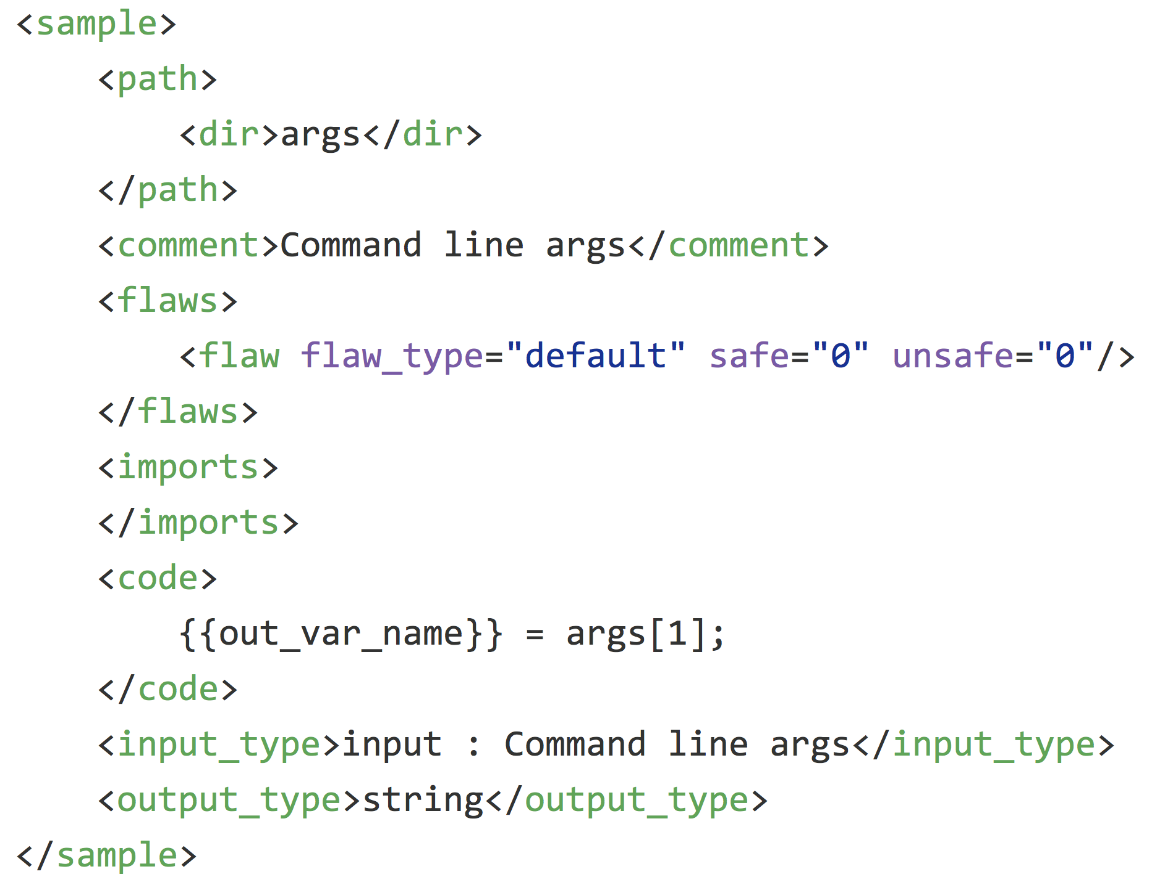
\includegraphics{fig_Input_file.png}
  \caption{Example Input module.  Instantiated at line 14 of 
  Fig.~\ref{fig:example main file}.}
  \label{fig:example input file}
\end{figure}

\begin{itemize}
    \item path: used in the file name. Each \texlangle dir\texrangle\ tag contains key words of the input method used. It is included in the file name. For example, when the key word in the \texlangle dir\texrangle\ tag is "none", the file name will contain ...I\_none\_..., where "I" is used to state the input selected
    
    \item flaw: the vulnerability categories where the sample can be used, e.g., if the input is compatible with a CWE and if it is safe for this CWE. For example, \\
    \verb|<flaw flaw_type="CWE_89" safe="0"/>| means that the input is for the CWE 89 and that it is not safe.  If an input is generic and compatible with all CWEs, put ``default'' in the ``flaw\_type'' attribute.

    \item input\_type: the type of input and its source.
    Declarations of \verb|variable| in the File Template give
    available types, see Sec.~\ref{sec: file template}.

    \item output\_type: the type of output.  The variable generated with the placeholder \\ \verb|{{out_var_name}}| in the code will be that type.

    \item code: The source code of an input. It should contain the placeholder \\ \verb|{{out_var_name}}|.  That placeholder will be replaced by the variable name used in the Filtering and Sink.  Do not declare this variable.
\end{itemize}

The case generated from the example Input in 
Fig.~\ref{fig:example input file}
takes an argument from the command line as Input.  
The input string can be either safe or unsafe, depending on user input.

\subsection{Filter Modules}

All filter modules are in the \verb|filtering.xml| file.

\begin{verbatim}
<sample>
    <path>
	    <dir></dir>
    </path>
    <comment></comment>
    <flaws>
	    <flaw flaw_type="" safe=""/>
    </flaws>
    <imports></imports>
    <code></code>
    <input_type></input_type>
    <output_type></output_type>
</sample>
\end{verbatim}

\begin{figure}[htbp]
  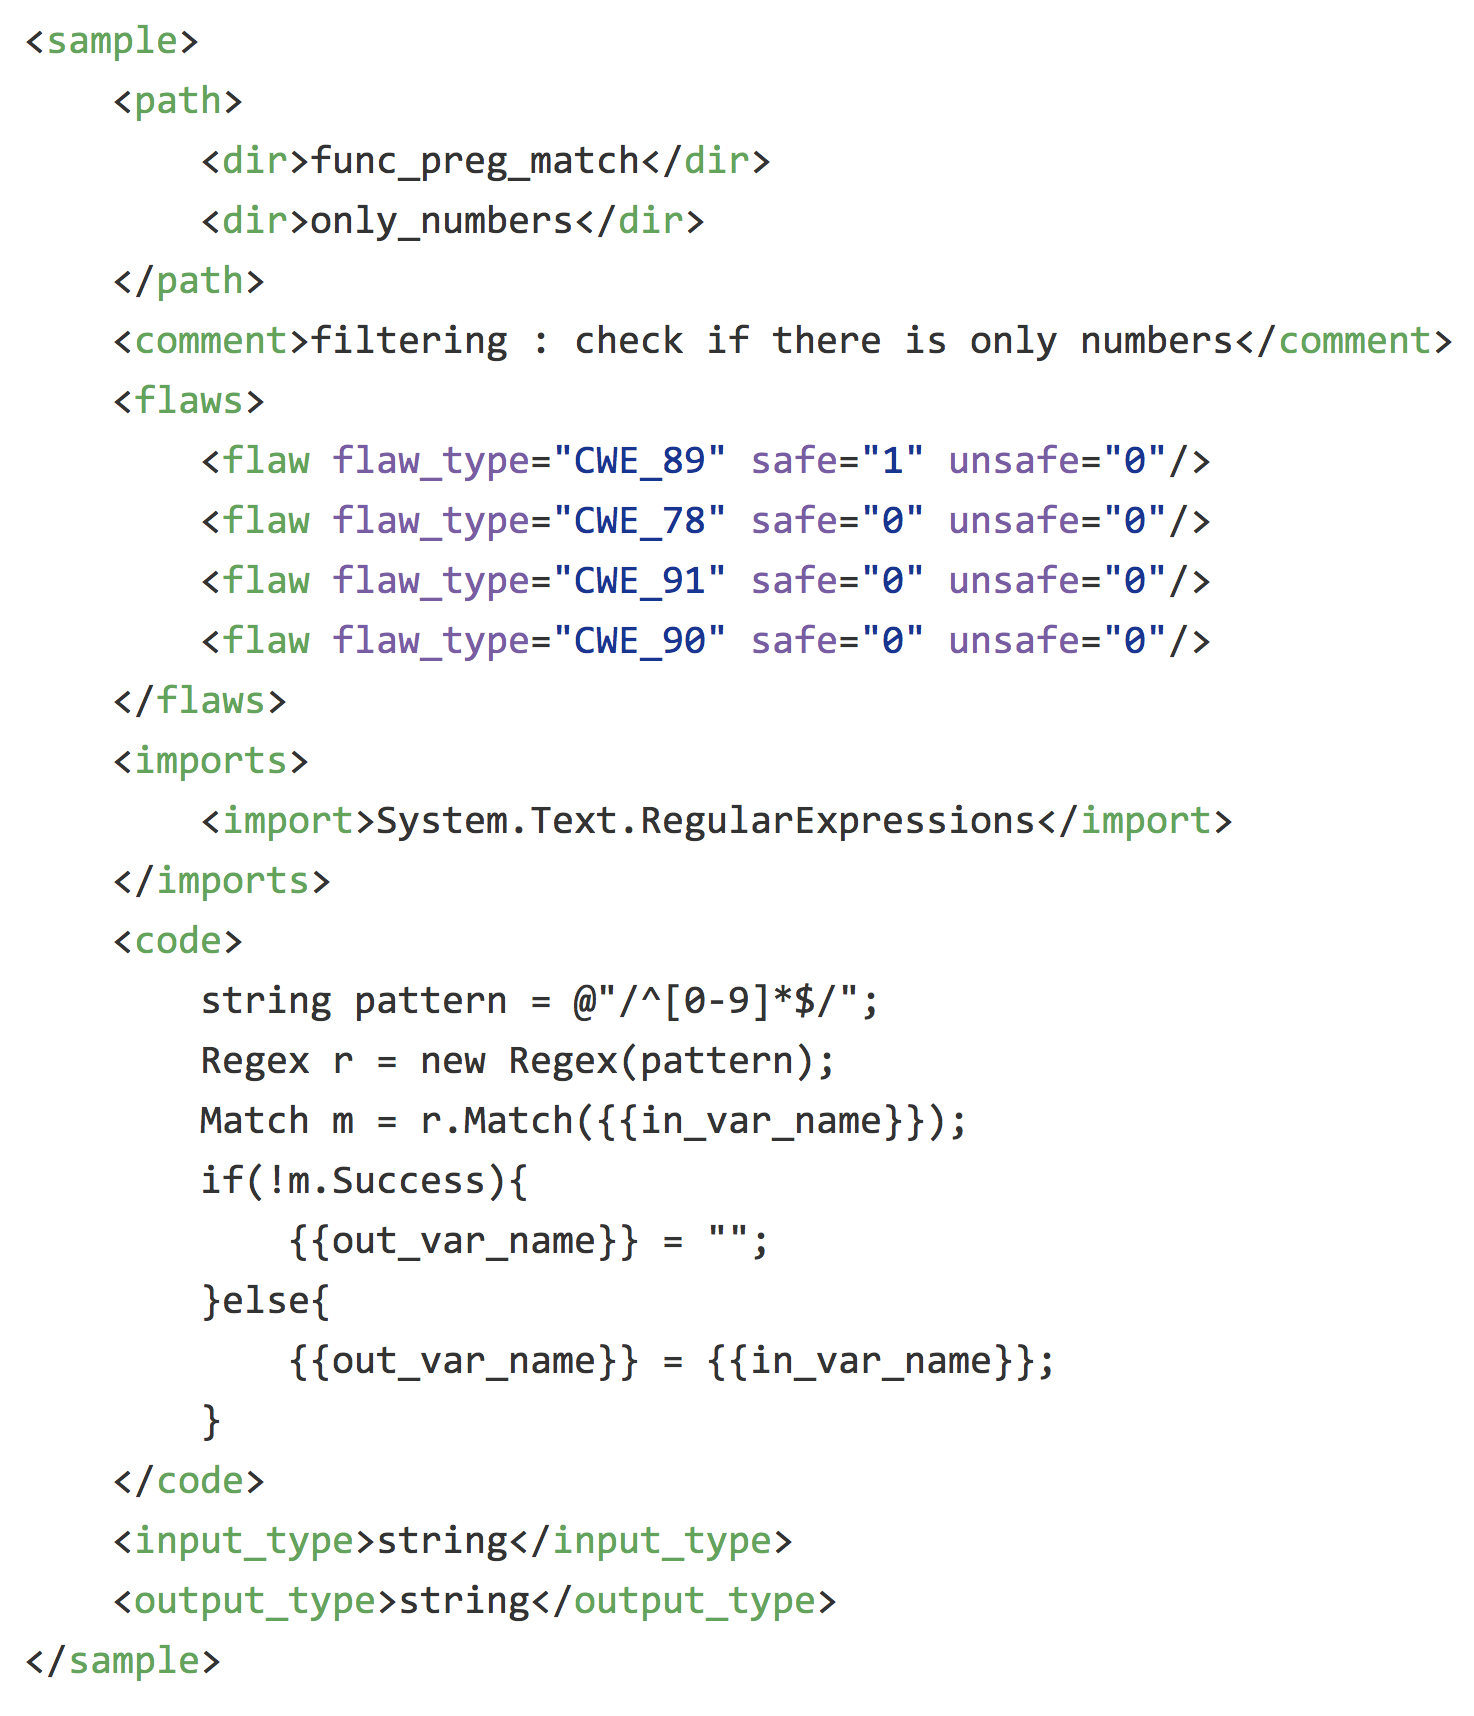
\includegraphics[width=\linewidth]{fig_Filter_file.png}
  \caption{Example Filter module. Instantiated in lines 19--27 of Fig.~\ref{fig:example aux file}.}
  \label{fig:example filter file}
\end{figure}

\begin{itemize}
    \item path: used in the file name.  Each \texlangle dir\texrangle\ 
    tag has
    key words of the filtering method used. It is used in the filename.
    
    \item input\_type: the input type of the filter. The variable 
    generated with
    the placeholder \verb|{{in_var_name}}| will be that type.
    Declarations of \verb|variable| in the File Template give
    available types, see Sec.~\ref{sec: file template}.

    \item output\_type: the output type of the filter.  The variable generated
    with the placeholder \verb|{{out_var_name}}| will be that type. \\
    Tip: To generate a test without Filtering, assign \verb|in_var_name| to
    \verb|out_var_name| and make the input\_type and output\_type \verb|nofilter|.
    This passes the variable from the Input directly to the Sink.

    \item flaw: whether the Filter is compatible with a CWE and if it is 
    safe for this CWE.  For example, \\
    \verb|<flaw flaw_type="CWE_89" safe="0"/>| means that the Filter is for 
    CWE 89 and that it is not safe.  Whereas \verb|safe=”1”| means that it is
    safe.  It could be safe for another CWE.  If a filter is compatible with all
    CWEs, put \verb|ALL| in the ``flaw\_type'' attribute.

    \item code: The source code of an filter. It should contain the placeholders
    \\
    \verb|{{in_var_name}}| and \verb|{{out_var_name}}|.  Those placeholders will 
    be replaced by the variable names used in the Input and Sink.  Do not declare 
    these variables.
\end{itemize}

The example Filter file in Fig.~\ref{fig:example filter file} makes sure
the Input contains only a number.  
The flag safe is 1, because you cannot cause an SQL Injection 
(CWE 89) with only numbers.


\subsection{Sink Modules}
\label{sec:sink modules}

All sink modules are in the language's \verb|sink.xml| file.

\begin{verbatim}
<sample>
    <path>
	    <dir></dir>
    </path>
    <flaw_type flaw_group=""></flaw_type>
    <safety safe="" unsafe=""/>
    <comment></comment>
    <imports>
        <import></import>
    </imports>
    <code></code>
    <input_type></input_type>
    <exec_type></exec_type>
</sample>
\end{verbatim}

\begin{itemize}
    \item flaw\_type: the flaw\_group is a general category of vulnerability.
    Generated test cases are placed under the flaw group subdirectory, then
    in the flaw type subdirectory under that. The user can limit
    cases generated to certain flaw groups with the \verb|-f| command
    line option or certain flaw types with the \verb|-c| option.
    
    \item input\_type: the input type of the sink. The variable
    generated with the placeholder \verb|{{in_var_name}}| will be 
    that type.  If the sink does not
    require an input, this type should be \verb|none|. The code 
    should not contain
    the placeholder \verb|{{in_var_name}}|.
    Declarations of \verb|variable| in the File Template give
    available types, see Sec.~\ref{sec: file template}.

    \item exec\_type: link a sink to the exec queries.  It must have 
    the type of
    an ExecQuery. If it does not require an ExecQuery, 
    exec\_type should be \verb|none|.

    \item safety: whether the sink is safe or not. If this sink is always
    ``safe'', assign a value of 1.  If always ``unsafe'', assign a value 
    of 1, so the file will be considered unsafe.  
    This is useful for a deprecated function.  If the Sink may be safe or 
    unsafe depending on the input and filtering, assign a value of 0 to 
    both attributes.  The safety of the generated case will depend on
    the Input and Filtering.
    
    \item code: The source code of a sink. It should contain the placeholder
    \verb|{{in_var_name}}|.  The placeholder will be replaced by the variable
    name used in the Filter.  Do not declare this variable.

    The placeholder \verb|{{flaw}}| indicates that the next line is the location
    of the flaw.  In other words, if this case is unsafe, the manifest reports a
    flaw at the number of the line following this.  In generated unsafe cases,
    \verb|{{flaw}}| is replaced with the one-line comment string,
    see Sec.~\ref{sec: file template}, and ``flaw''.
    It does not appear in generated safe cases.
    Note: the generated code shown in Fig.~\ref{fig:example main file} is incorrect:
    it does not show the \verb|//flaw| line that would be generated.
\end{itemize}

\begin{figure}[htbp]
  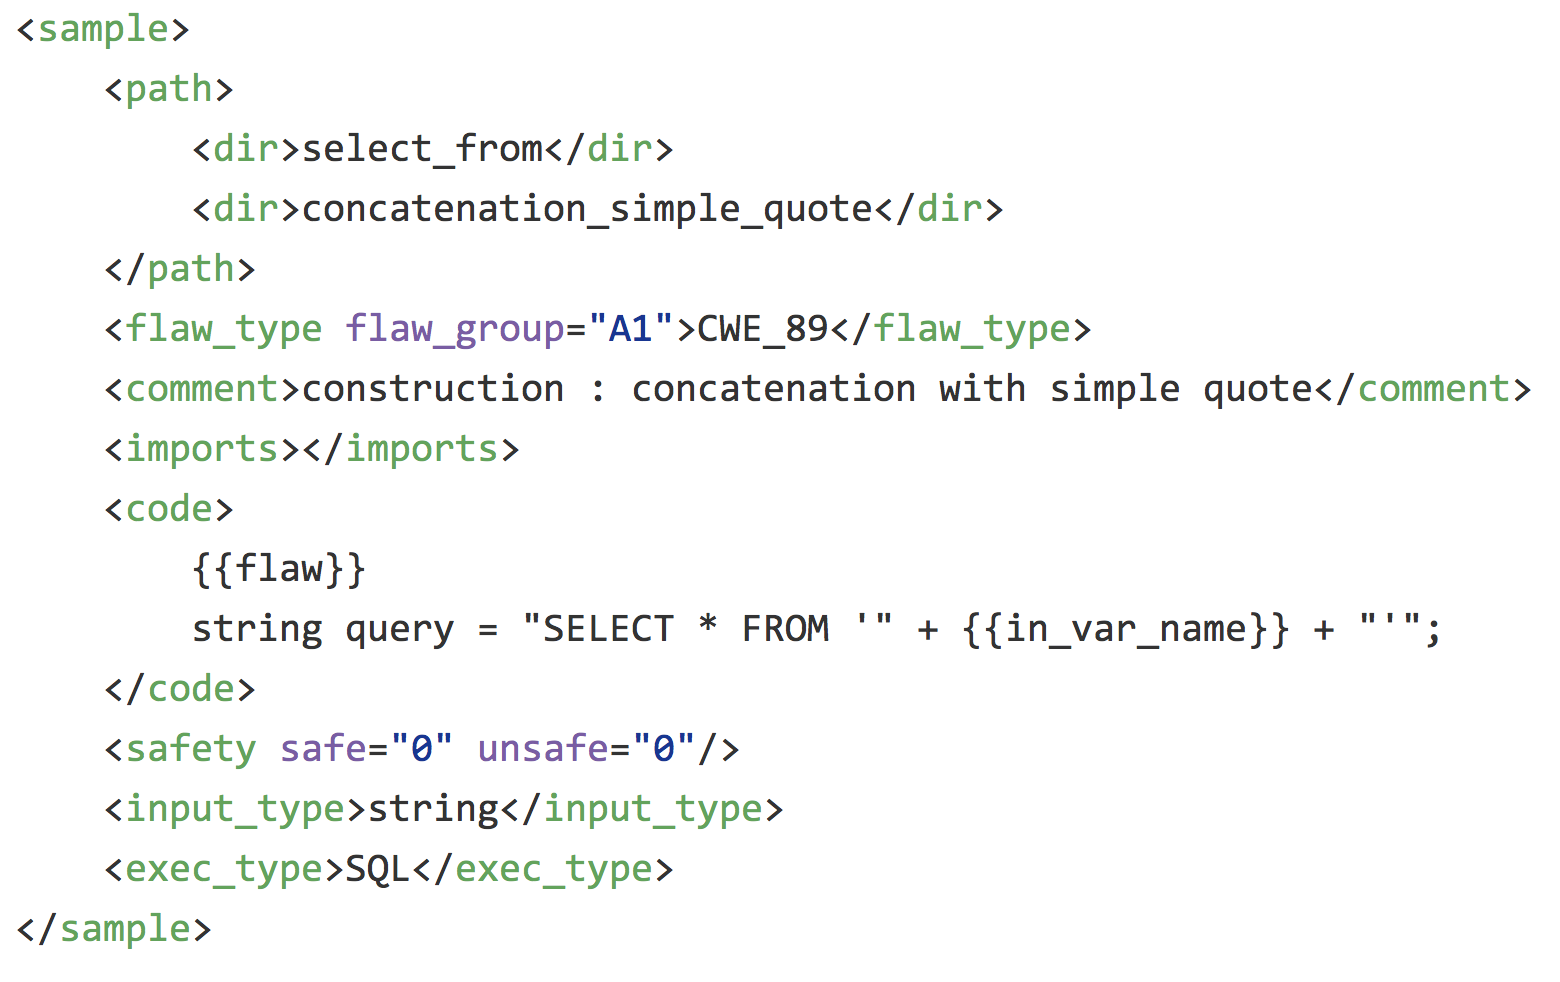
\includegraphics[width=\linewidth]{fig_Sink_file.png}
  \caption{Example Sink module. Instantiated at line 23 of Fig.~\ref{fig:example main file}.}
  \label{fig:example sink file}
\end{figure}

The Sink example in Fig.~\ref{fig:example sink file} 
concatenates the filtered string with a SQL query.  This block 
of code can only be used for SQL Injection.  Whether or not it is
vulnerable depends on the input string.


\subsection{Exec\_Query Modules}

All query execution(??) modules are in the language's \verb|exec_query.xml|
file.

\begin{verbatim}
<exec_query type="" safe="">
    <path>
	    <dir></dir>
    </path>
    <comment></comment>
    <imports>
        <import></import>
    </imports>
    <code></code>
</exec_query>
\end{verbatim}

\begin{itemize}
    \item type: the type of the ExecQuery. This type is used in the 
    \verb|exec_type| tag of the Sink in order to link them together during
    generation process.  The type should only contain letters, numerals, and
    underscore (``\_'').\\
    VTSG V3 supports many database management systems, including ORACLE, \\
    MySQL,
    MSSQL, Postgre, SQLite, and XPATH.  The syntax of each ExexQuery must be
    compatible with its associated database system language.
    
    \item safe: whether the ExecQuery makes the case safe or not.

    \item code: The source code of a query. It does not contain placeholders.
    It should be linked to the corresponding variable from the Sink. The linking is done through the "exec\_type" attributes within the XML files.
\end{itemize}


\begin{figure}[htbp]
  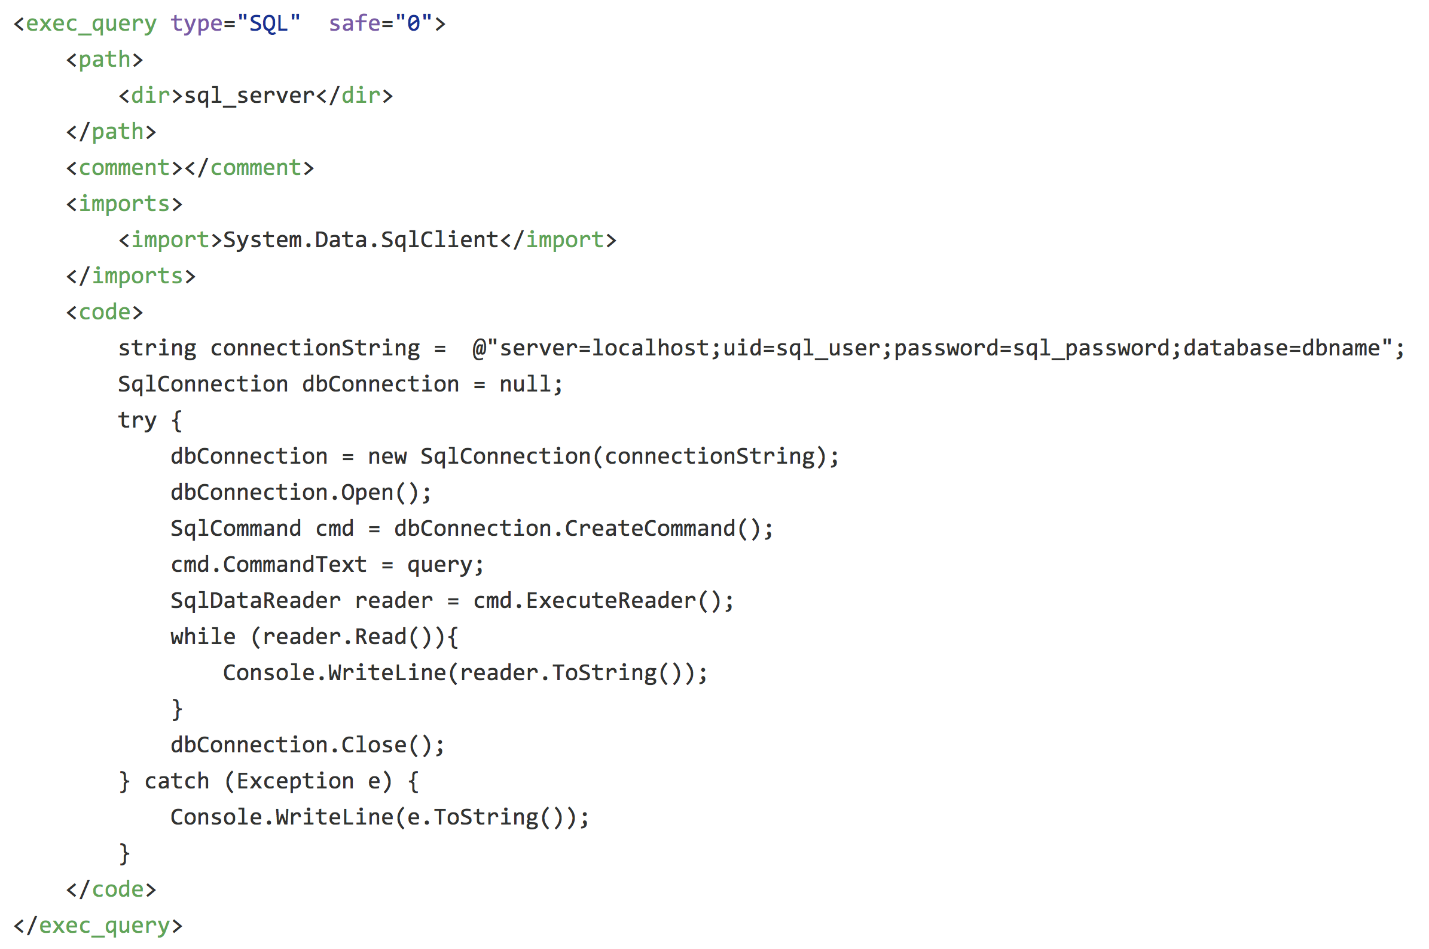
\includegraphics[width=\linewidth]{fig_Exec_Query_file.png}
  \caption{Example Exec\_Query module. Instantiated in lines 25--39 of
    Fig.~\ref{fig:example main file}.}
  \label{fig:example exec-query file}
\end{figure}

The block of code in the Exec\_Query example, 
Fig.~\ref{fig:example exec-query file}, executes the SQL query, used 
for database management
systems, including MySQL, Oracle, Postgre, and SQLite.  This example is 
vulnerable.  If a non-vulnerable execution of a SQL query is required, 
use a SQL prepared statement.


\subsection{Test Condition and Code Complexity Modules}

All test condition and code complexity modules are in the 
language's \verb|complexities.xml| file.  This file has
a \verb|<root>| with one \verb|<conditions>| and one
\verb|<complexities>|.
All condition modules are inside \verb|<conditions>|.  All
complexity modules are inside \\ \verb|<complexities>|.

\begin{verbatim}
<root>
    <conditions>
        <condition ...>
            ...
        </condition>
        ....
    </conditions>
    <complexities>
        <complexity ...>
            ...
        </complexity>
        ....
    <complexities>
\end{verbatim}

\subsubsection{Test Condition Modules}
\label{sec: condition modules}

\begin{verbatim}
<condition id="">
    <code></code>
    <value></value>
</condition>
\end{verbatim}

\begin{itemize}
    \item id: Unique string(?) for the Condition.  Appears in
    the test case file name.
    
    \item code: the source code of the conditional test.

    \item value: either \verb|<value>True</value>| or
        \verb|<value>False</value>| depending on \\
        whether the code evaluates to true or false.
\end{itemize}

\begin{figure}[htbp]
  % width makes the text about the same size as text in Complexity_file_while
  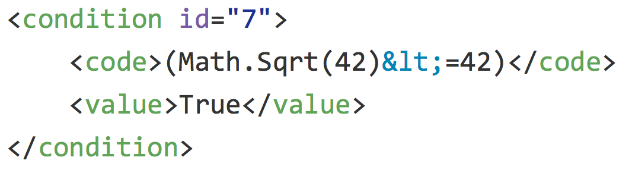
\includegraphics[width=2.4in]{fig_Complexity_file_test.png}
  \caption{Example test condition module.  Instantiated in
    Fig.~\ref{fig:example main file}, line 16.}
  \label{fig:example complexity-test file}
\end{figure}


\subsubsection{Code Complexity Modules}
\label{sec: complexity modules}

\begin{verbatim}
<complexity id="" type="" group="" executed="" in_out_var="i" 
                                         indirection="" need_id="">
    <code></code>
	<body></body>
</complexity>
\end{verbatim}

\begin{itemize}
    \item id: Unique string(?) for the Complexity.  This is at the 
    end of the
    name of the generated file.

    \item type: Supported types are: \verb|if|, \verb|switch|, \verb|goto|, 
    \verb|for|, \verb|foreach|, \verb|while|, \\
    \verb|function|, and \verb|class|.

    \item group: Supported groups are: \verb|conditionals|, \verb|jumps|, 
    \verb|loops|, \verb|functions|, and \\ \verb|classes|.

    \item executed: whether the placeholder will be executed or not. Four 
    values are allowed:
    \begin{itemize}
        \item 0: Not executed
        \item 1: Executed
        \item condition:  Executed if the condition is true
        \item not condition:  Executed if the condition is false
    \end{itemize}

    \item in\_out\_var: whether the variable (from the Input) will be used or
    transformed in the Complexity before being used in the Filter.  If the
    variable is neither used nor transformed, do not use this attribute.
    Three values are allowed:
    \begin{itemize}
        \item in: the variable is used before the placeholder 
        \item out: the variable is used after the placeholder
        \item traversal: the variable is used in the placeholder
    \end{itemize}
    If this attribute is used, the code should contain the following 
    placeholders: \\
    \verb|{{in_var_name}}|, \verb|{{out_var_name}}|, and \verb|{{var_type}}|.

    \item indirection: ``1'' if the code is split into two chunks (call and
    declaration) or calls a function.  The body tag should be present when 
    calling a function.

    \item need\_id: ``1'' if the code has a placeholder, \verb|{{id}}|,
    to generate a unique ID for the Complexity.  This ID to generate 
    a label, a parameter, or a function name in a nested
    context.

    \item code: the source code of the Complexity.  Code or 
    body should contain the placeholder, \verb|{{placeholder}}|, 
    where the Filter is inserted.  It may contain the
    placeholder, \verb|{{condition}}|, where the Condition 
    is inserted.

    \item body:  Contains the source code not in the main execution 
    flow, e.g., 
    functions or classes. (optional)
\end{itemize}


\begin{figure}[htbp]
  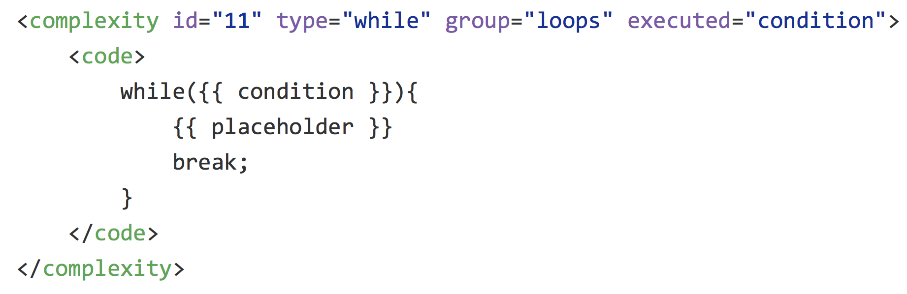
\includegraphics[width=4in]{fig_Complexity_file_while.png}
  \caption{Example Complexity module with a {\texttt while} loop.  Instantiated in 
    Fig.~\ref{fig:example main file}, lines 16--21.}
  \label{fig:example complexity-while file}
\end{figure}

\begin{figure}[htbp]
  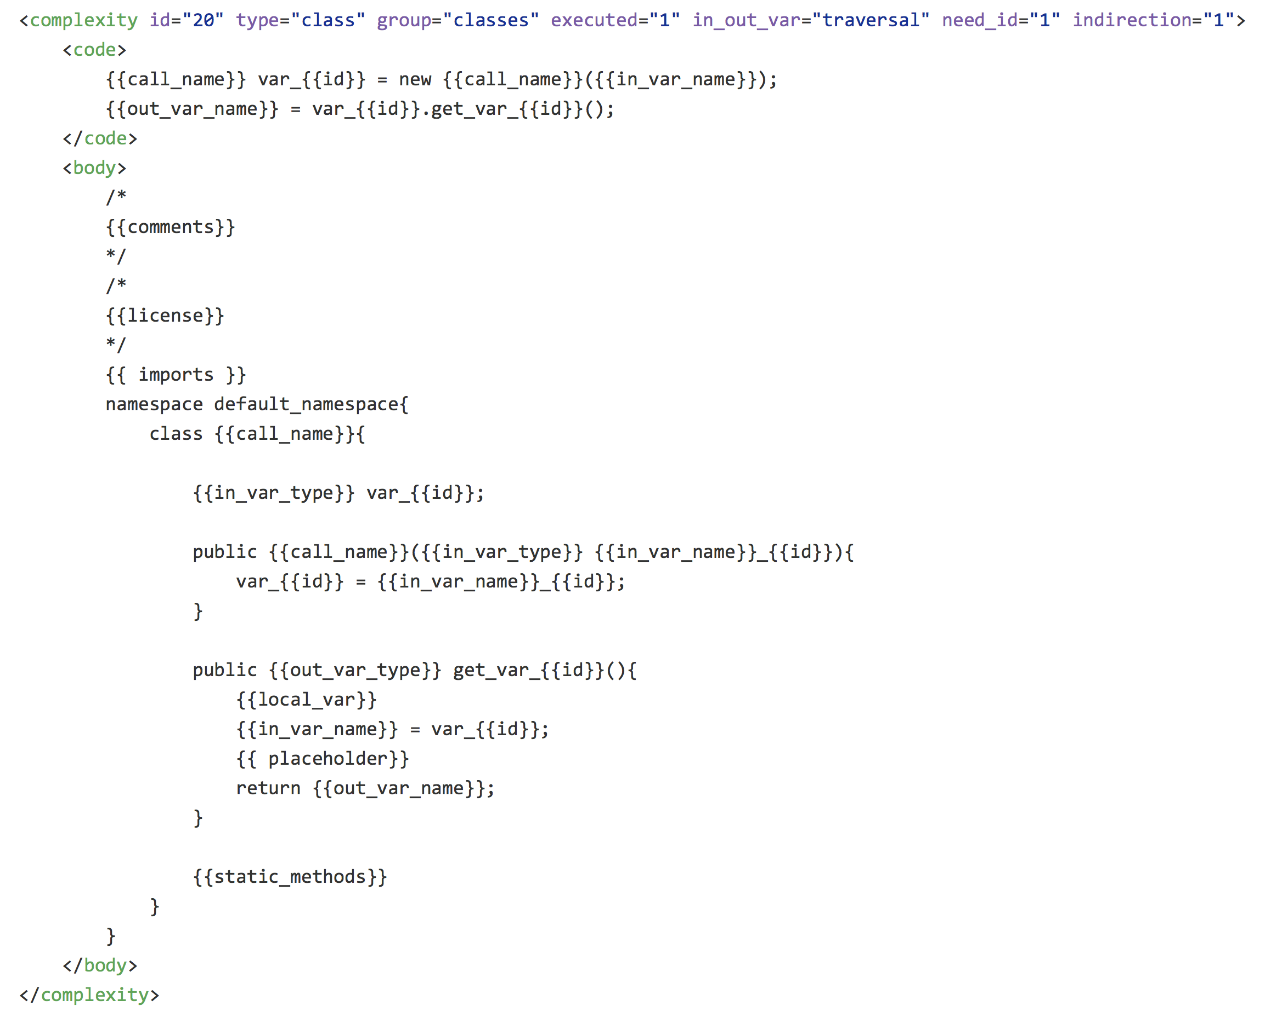
\includegraphics[width=\linewidth]{fig_Complexity_file_method.png}
  \caption{Example Complexity module with a method invocation.  
  The \texlangle code\texrangle\ part is instantiated in
  Fig.~\ref{fig:example main file}, lines 18 and 19. 
  The \texlangle body\texrangle\ part is instantiated in
  Fig.~\ref{fig:example aux file}.}
  \label{fig:example complexity-method file}
\end{figure}

When adding Complexity, VTSG can use several complexity in one
test case.
The example in Sec.~\ref{sec:generated files} has two types of
Complexity: a control flow complexity and a data flow complexity. 
The control flow complexity specification is in 
Fig.~\ref{fig:example complexity-while file}.  It is instantiated in 
lines 16--21 of
Fig.~\ref{fig:example main file}.  Line 16 is the instantiation of 
the control flow condition
specified in Fig.~\ref{fig:example complexity-test file}.

The data flow complexity is a method call within the \verb|while| loop.  
The specification
is in Fig.~\ref{fig:example complexity-method file}.  
The \texlangle code\texrangle\ 
part is instantiated in lines 18 and 19 of 
Fig.~\ref{fig:example main file}. 
The \texlangle body\texrangle\ part is instantiated in 
Fig.~\ref{fig:example aux file}.


\section{Generated Test Cases}

This section describes where VTSG places test cases and what the
names of test case files mean.

\subsection{Directory Structure of Generated Test Cases}
\label{sec: test suite directory structure}

 a description of the directory structure where test cases are placed.

\subsection{Test Case File Names}
\label{sec:case file name}

VTSG names test case files as
\verb|cwe_NB__I_INPUT__F_FILTER__S_SINK__EQ_EXEC_| \\
\verb|QUERY__NBCPLX-CPLX1-CPLX2.COND_FileX.EXT|
\begin{itemize}
    \item NB:  CWE number (two or three digits)
    \item INPUT:  Input name (optional)
    \item FILTER:  Filter name (optional)
    \item SINK:  Name of the critical function
    \item EXEC\_QUERY:  ExecQuery name (optional)
    
    \item NBCPLX:  The number of complexities. Each complexity has the tags 
    \begin{itemize}
        \item CPLX1, CPLX2, \ldots: ID given in 
            code complexity modules, 
            see Sec.~\ref{sec: complexity modules}. 
            Table~\ref{tab:complexity IDs} in the appendix 
            lists complexitie IDs currently used with 
            PHP or \CSharp.
            (optional)
        \item COND: ID given in test condition modules,
            see Sec.~\ref{sec: condition modules}.
            Table~\ref{tab:condition IDs} lists condition 
            IDs currently used. (optional)
    \end{itemize}
    \item X: Number of the file within the test. 
    1 is the main file. 2, 3, 
    \ldots are other files, such as classes. {\Large Juliet uses a, b, c, d}
    \item EXT: file extension
\end{itemize}

Example
\verb|cwe_89__I_args__F_func_preg_match-only_numbers__S_select_| \\
\verb|from-concatenation_simple_quote__EQ_mysql__1-2.4_File1.cs|

The Complexity part near the end, 1-2.4, means there is one Complexity. 
It is complexity 2 with condition 4.

File names reflect the entire case, not just the code in a 
particular file.  The
example in Sec.~\ref{sec:generated files} shows that both 
files of the case have
identical names, except for the final FileX part.

\section{Example Test Case}
\label{sec:generated files}

\begin{figure}[htbp]
  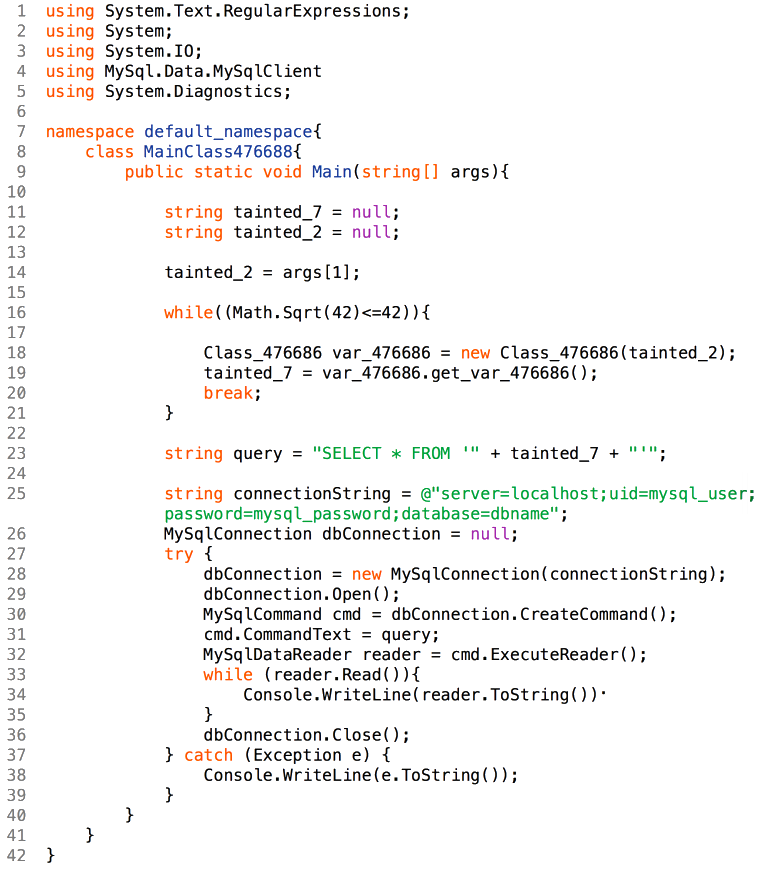
\includegraphics[width=\linewidth]{fig_example_code1.png}
  \caption{Main file of example. Line 14 instantiates input code from 
    Fig.~\ref{fig:example input file}. Lines 16--19 instantiates complexity code from 
    Fig.~\ref{fig:example complexity-while file}. Line 16 instantiates condition code from
    Fig.~\ref{fig:example complexity-test file}.  Lines 18 and 19 instantiate code from the
    \texlangle code\texrangle\ part of Fig.~\ref{fig:example complexity-method file}.
    Line 23 instantiates critical preparation code from Fig.~\ref{fig:example sink file}.
    Lines 25--39 instantiate query execution code from Fig.~\ref{fig:example exec-query file}.
    Note: a //flaw line would be generated before line 23.
  }
  \label{fig:example main file}
\end{figure}

\begin{figure}[htbp]
  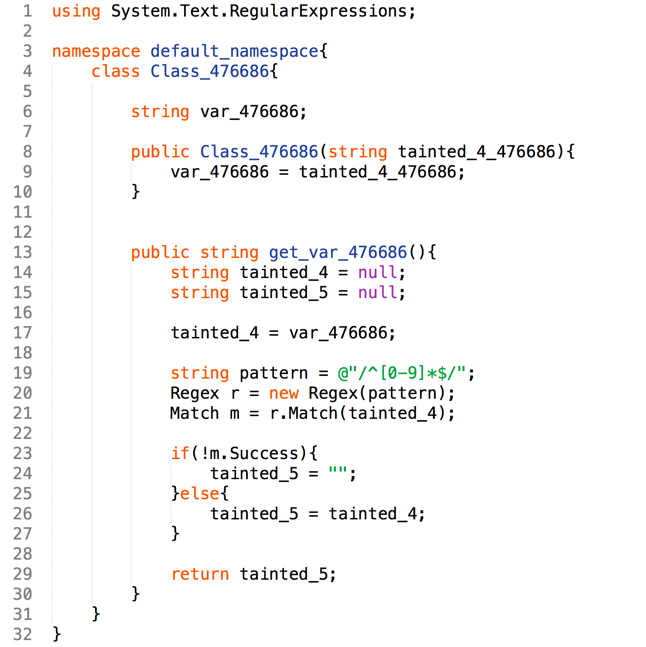
\includegraphics[width=0.85\linewidth]{fig_example_code2.png}
  \caption{Auxiliary file of example.  It instantiates code from the \texlangle body\texrangle\ 
    part of Fig.~\ref{fig:example complexity-method file}.  Lines 19--27 instantiate filter code
    from Fig.~\ref{fig:example filter file}.}
  \label{fig:example aux file}
\end{figure}

This section has an example test case.  The case consists of 
two files.
Fig.~\ref{fig:example main file} is the main file of the example.  
Fig.~\ref{fig:example aux file} is an auxiliary class file.  
The code in
the main file invokes the class at line 18.

The name of the main file is
\verb|cwe_89__I_shell_commands__F_func_preg_| \\
\verb|match-only_numbers__S_select_from-concatenation_simple_quote__| \\
\verb|sql_server__2-11.7-20_File1.cs|.
The name of the class file, Fig.~\ref{fig:example aux file}, is
identical, except for the
file number, ``2''.

Using Sec.~\ref{sec:case file name}, Table~\ref{tab:complexity IDs}, and
Table~\ref{tab:condition IDs}, the file name can be understood as follows:

\noindent CWE 89: Improper Neutralization of Special Elements used in an SQL Command ('SQL Injection')\cite{CWE89}

\noindent Input	shell\_commands, see specification in Fig.~\ref{fig:example input file}

\noindent Filter  func\_preg\_match-only\_numbers, Fig.~\ref{fig:example filter file}

\noindent Sink	select\_from-concatenation\_simple\_quote\_\_sql\_server, 
Fig.~\ref{fig:example sink file}.

\noindent Complexities 2-11.7-20  two complexities; 11 = \verb|while|,
Fig.~\ref{fig:example complexity-while file}, 
with condition 7 = \verb|Math.| \verb|Sqrt(42)<=42|: True, Fig.~\ref{fig:example complexity-test file}; and
20 = class traversal executed, Fig.~\ref{fig:example complexity-method file}.

\noindent File1 main file

\noindent The extension, cs, shows that it is a \CSharp\ file.



\section{Acknowledgements}

Bertrand Stivalet and Aurelien Delaitre, from the NIST SAMATE team, designed the
architecture of the VTSG project and managed its implementation.  The project was
implemented by students from TELECOM Nancy: Jean-Philippe Eisenbarth, Valentin
Giannini, and Vincent Noyalet.  We thank Terry Cohen for her comments and
suggestions, which improved this report.  We also thank Elizabeth Fong and
Charles de Oliveira for their contributions to this report.
% On 12 June 202, Terry Cohen wrote [[much editing by PEB]]
% Bertrand and Liz wrote the original document. I did some quick grammatical editing. Liz submitted it, but Barbara wanted it to cover both C# and PHP. The original did not have both. Because of the SATE V and CSIAC projects, this was put on hold.
%
% As I revised the NIST IR, I went through all of the instructions to verify the PHP statistics in the paper that Bertrand and Liz published and to generate C# statistics. I discovered errors and/or missing commands in the instructions. Charles pointed out the missing instructions.
%
% I recommend crediting Bertrand and Liz, because they started documentation. Although I wrote the new documents covering both C# and PHP, I know that Will and Carin will add Python.  I do not need to have my name on the new project.
%
% I added Charles because he helped me find the missing commands.  At the time, he was indifferent to being listed as a co-author.  We were using it as a learning exercise.
%
% In summary, I recommend that Bertrand, Liz, you, and your team be listed as co-authors.


% references section
\addcontentsline{toc}{section}{References}
\bibliographystyle{techpubs}
\bibliography{vulTestSuiteGenV3}

\newpage

%%%%%%%%%%%%%%%%%%%%%%%%%%%%%%%%%%%%%%%%%%%%%%%%%%%%%%%%%%%%%%%%%%%%%
%
%           APPENDIX
%
%%%%%%%%%%%%%%%%%%%%%%%%%%%%%%%%%%%%%%%%%%%%%%%%%%%%%%%%%%%%%%%%%%%%%

% make the Appendix begin on a new page (not a new column) even in
% two-column mode
\clearpage

\appendix

\section{Complexity and Condition IDs}
\label{sec: complexity and condition IDs}

This section lists complexities and conditions currently
available for \CSharp\ and PHP.
We explain code complexities in Sec.~\ref{sec:code complexities}.

%\subsection{This is a Subsection in the Appendix}

\begin{table}[H]
\centering
\begin{tabular}{|r|l|}
\hline
\textbf{ID} & \textbf{Complexity} \\
\hline
 1 & if condition \\
\hline
 2 & if condition \\
\hline
 3 & if not condition \\
\hline
 4 & if condition \\
\hline
 5 & if not condition \\
\hline
 6 & if condition \\
\hline
 7 & if not condition \\
 \hline
 8 & if not executed \\
\hline
 9 & switch executed \\
\hline
10 & switch not executed \\
\hline
11 & while condition \\
\hline

12 & do while executed \\
\hline
13 & for executed \\
\hline
14 & foreach executed \\
\hline
15 & goto not executed \\
\hline
16 & goto executed \\
\hline
17 & function traversal executed \\
\hline
18 & function in executed \\
\hline
19 & function out executed \\
\hline
20 & class traversal executed \\
\hline
21 & class in executed \\
\hline
22 & class out executed \\
\hline
\end{tabular}
\caption{Complexity IDs Defined for \CSharp\ and PHP}
\label{tab:complexity IDs}
\end{table}

{\Large Why are they four ``if condition''s? (and three ``if not condition''s)}

{\Large What does ``condition'' mean vs. ``executed''?}

{\Large Explain connection between table and code and body.}

Complexities are defined in Code Complexity Modules, see
Sec.~\ref{sec: complexity modules}.

\begin{table}[H]
\centering
\begin{tabular}{|r|l|l|}
\hline
\textbf{ID} & \textbf{Code} & \textbf{Value} \\
\hline
1 & \verb|1==1| & True \\
\hline
2 & \verb|1==0| & False \\
\hline
3 & \verb|4+2<=42| & True \\
\hline
4 & \verb|4+2>=42| & False \\
\hline
5 & \verb|Math.Pow(4, 2)<=42| & True \\
\hline
6 & \verb|Math.Pow(4, 2)>=42| & False \\
\hline
7 & \verb|Math.Sqrt(42)<=42| & True \\
\hline
8 & \verb|Math.Sqrt(42)>=42| & False \\
\hline
\end{tabular}
\caption{Condition IDs Associated with Complexities in Table~\ref{tab:complexity IDs}}
\label{tab:condition IDs}
\end{table}

The value indicates that the code always evaluates to true or false,
respectively.
Conditions are defined in Test Condition Modules,
see Sec.~\ref{sec: condition modules}.

{\Large Can any condition go with any complexity?}

\end{document}
